\section{Results}
The machined part was created as shown in Figure \ref{fig:result}
\begin{figure}[h!]
	\centering
	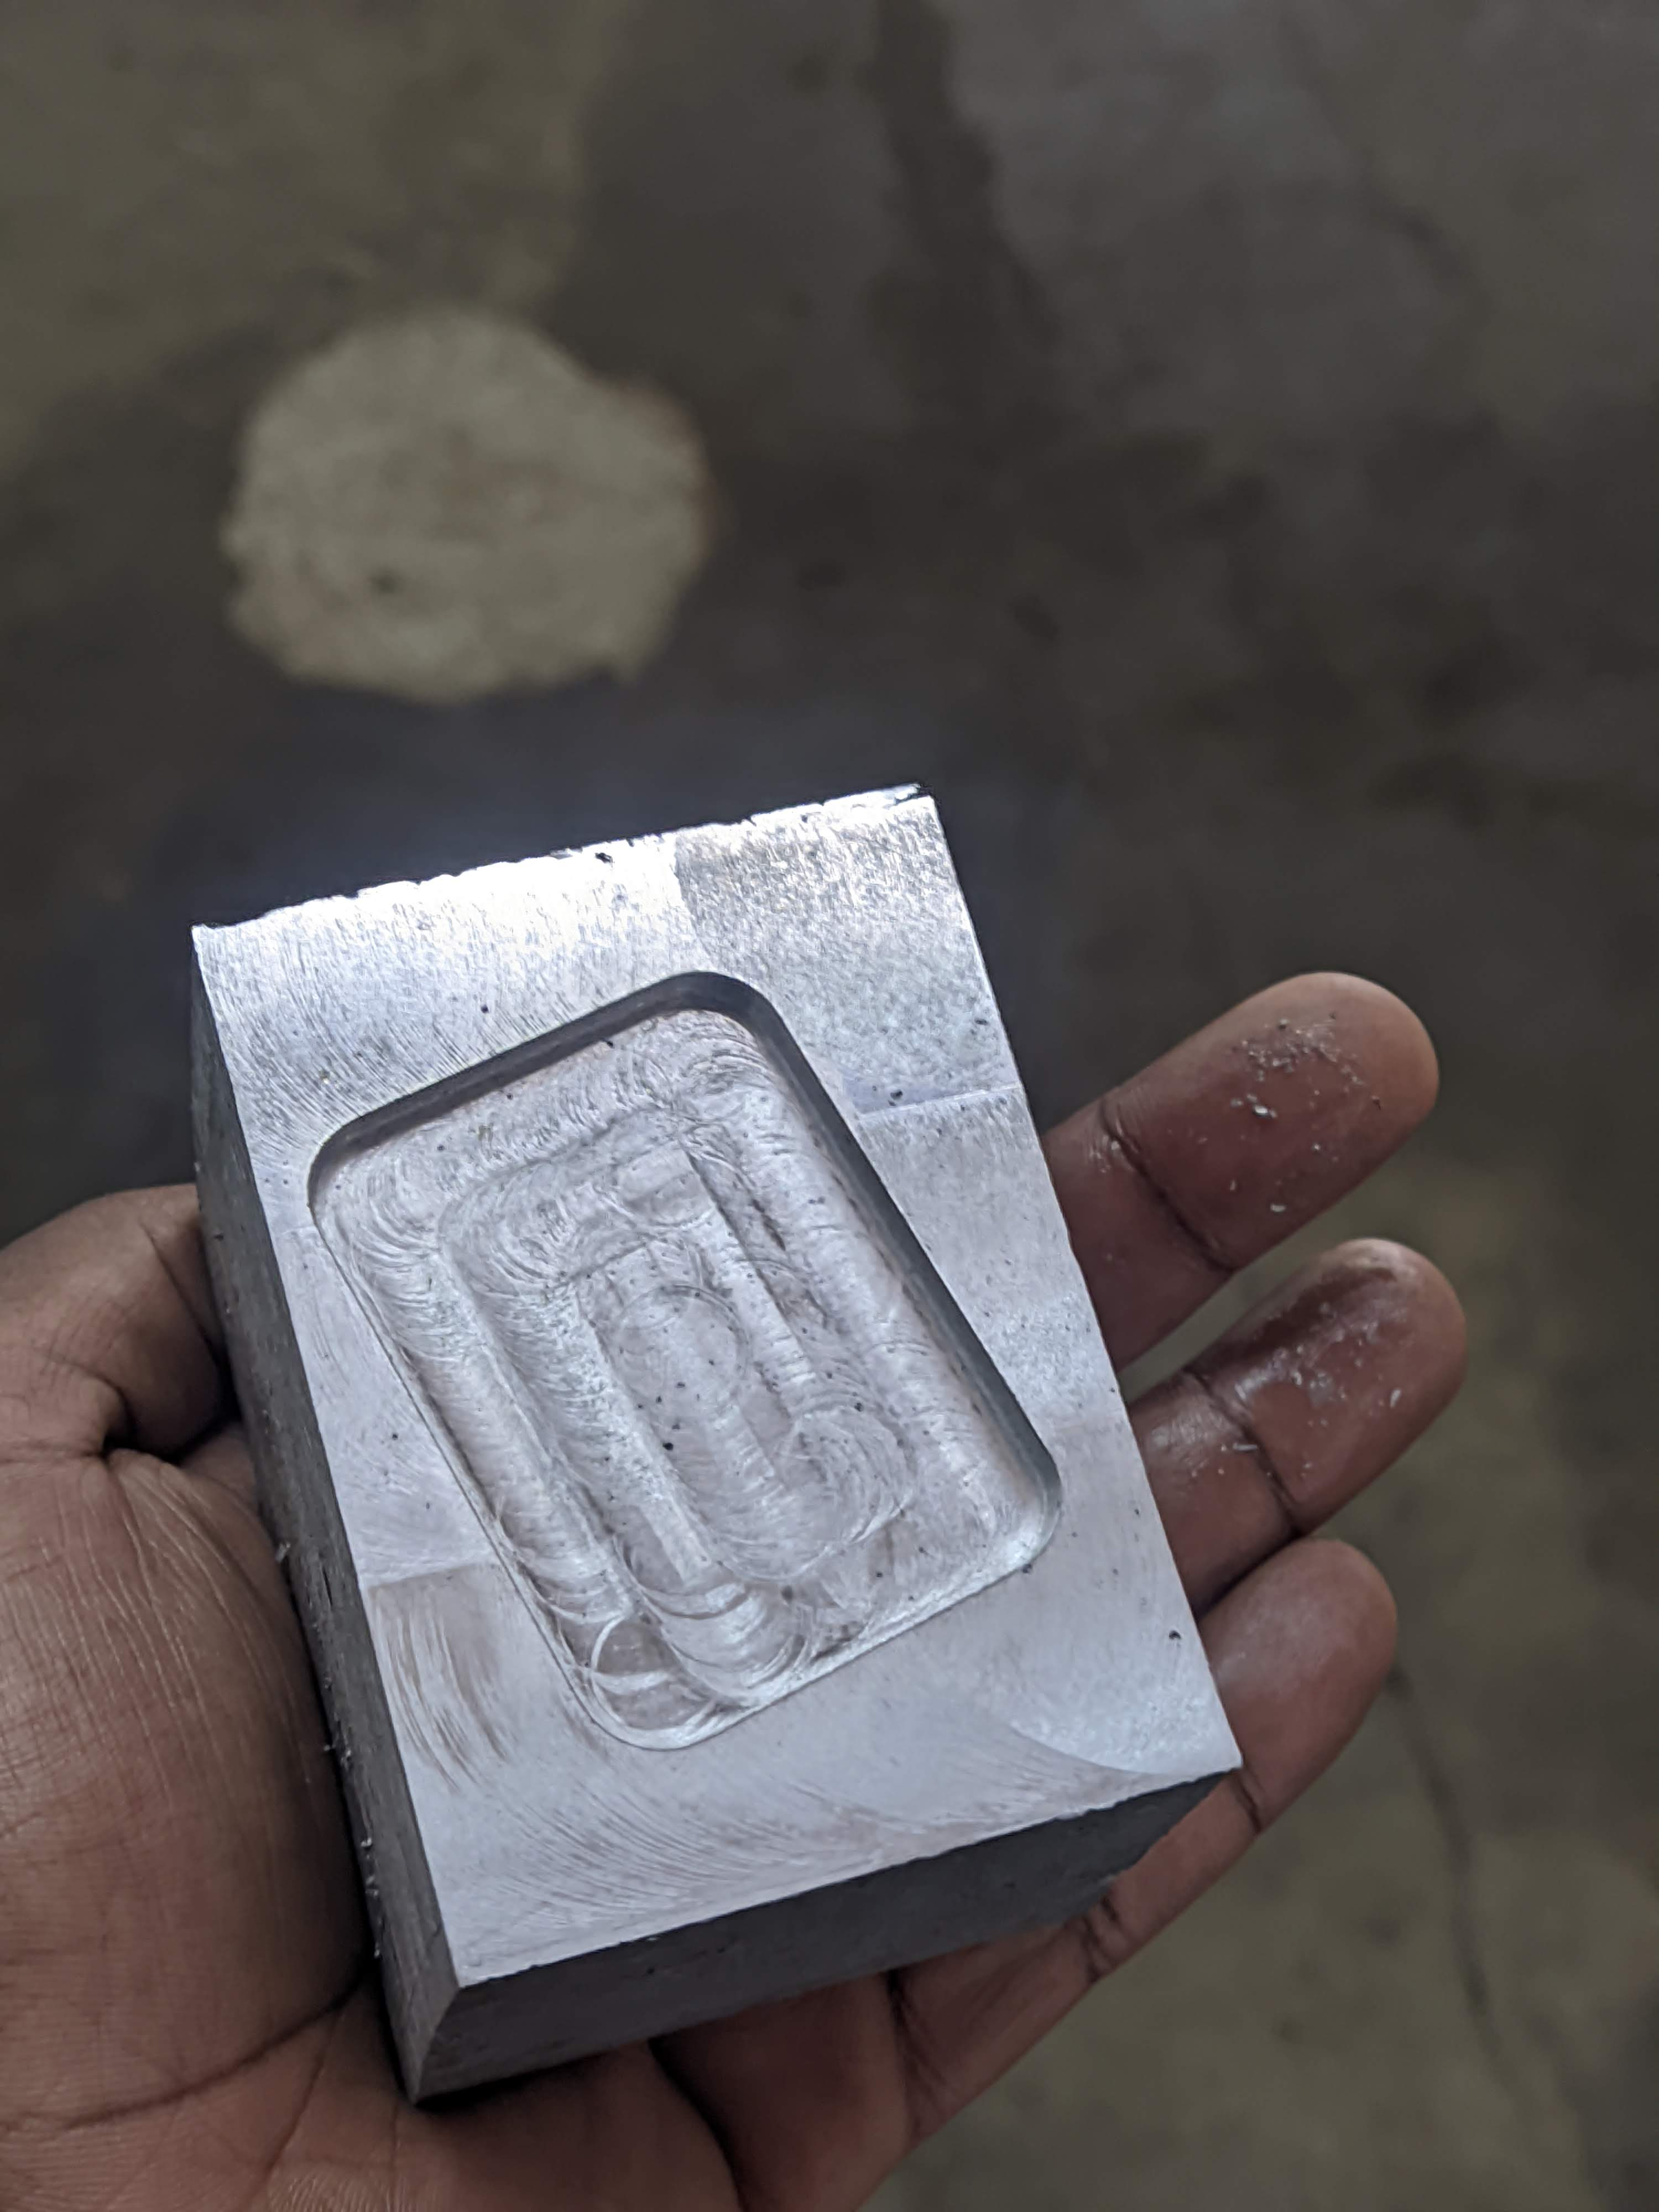
\includegraphics[width=0.8\linewidth]{Figures/result}
	\caption[Result]{The Machined Part}
	\label{fig:result}
\end{figure}
The operations done were:
\begin{enumerate}
	\item Face Milling
	\item Pocket milling
\end{enumerate}

\section{Discussion}
\subsection{CNC Machining}
The machining operation was successfully carried out and the workpiece retrieved. G- and M-codes were used in manual part programming. These codes are specific to the CNC machine and are specified by the manufacturer. The CNC Machine M-code list is shown in the appendix.\\